\documentclass[12pt]{report}
\usepackage[utf8]{inputenc}
\usepackage{amsmath}
\usepackage{amsfonts}
\usepackage{amssymb}
\usepackage{graphicx}
\usepackage{caption}
\usepackage{booktabs}
\usepackage{hyperref}
\usepackage{csquotes}
\usepackage{indentfirst}
%
\title{Modeling Human Visual System in Patch-base Image Quality Assessment using Deep Learning}	%% title
\author{Nguyen Trung Nghia}			%% author's name

%
\newcommand{\argmax}{\arg\!\max}

\begin{document}
%
\maketitle

%
\chapter*{Authorship}
“I hereby declare that the work contained in this thesis is of my own and has not been
previously submitted for a degree or diploma at this or any other higher education
institution. To the best of my knowledge and belief, the thesis contains no materials
previously published or written by another person except where due reference or
acknowledgement is made.”

Signature: .................

%
\chapter*{Supervisor’s approval}

“I hereby approve that the thesis in its current form is ready for committee examination
as a requirement for the Bachelor of Computer Science degree at the University of
Engineering and Technology.”
\newline
Signature: .................


\chapter*{Acknowledgement}

I am grateful to thank the Department of Computational Science and Engineering, and HMI Lab both at the VNU UET for the support.

I would like to express our sincere thanks to our advisor Ph.D. Le Thanh Ha and M.Sc. Pham Thanh Tung for their support and guidance throughout this research work.
%
\chapter*{Abstract}

As humans are the ultimate receivers of the majority of visual signals being processed, the most accurate way of assessing image quality is to ask humans for their opinions of an image’s quality, known as the subjective visual quality assessment (VQA). The subjective image quality scores gathered from all subjects are processed to be the mean opinion score (MOS), which is regarded as the ground truth of image quality. Conventionally, a number of full-reference image quality assessment (FR-IQA) methods adopted various computational models of the human visual system (HVS) from psychological vision science research.

Due to the fact that the human visual system (HVS) is differently sensitive to features of image patch, we propose Deep Image Patch Quality Assessment (DIPQA), a novel image patch quality assessment that used deep neural network-based approach. An experimental quality assessment to approach database for image patch has been developed. The network is train end-to-end and comprises 8 convolutional layers and 4 pooling layers for feature extraction, and 2 fully connected layers for regression, which make it significantly deep enough to learn the mean opinion score (MOS) of the developed dataset.

We promise that this project was contributed by all members in our group, which are supervised by Ph.D. Le Thanh Ha and M.Sc. Pham Thanh Tung from HMI Lab. The report contains no materials previously published or written by another person except where due reference or acknowledgement is made.
%
\tableofcontents
\listoffigures
\listoftables

\chapter*{Abbrevations}
%
\chapter{Introduction}

With the growing popularity of smartphones, compact cameras, and Internet services such as Facebook and Instagram, the production and sharing of digital images has grown tremendously over the past few years.  
The Fig.\ref{fig:digimgs} show the journey of a picture begins with it being obtained by a camera, which changes over it into a digital format and compresses it utilizing lossy compression algorithms to meet the onboard storage accessibility. 
This image is then transmitted over wired or wireless transmission channels and is altered in its resolution to meet the available bandwidth. 
Finally, the end user receives this image and watches it over devices ranging from smartphones to 4K displays, which require further alterations to its resolution. 

\begin{figure}[H]
  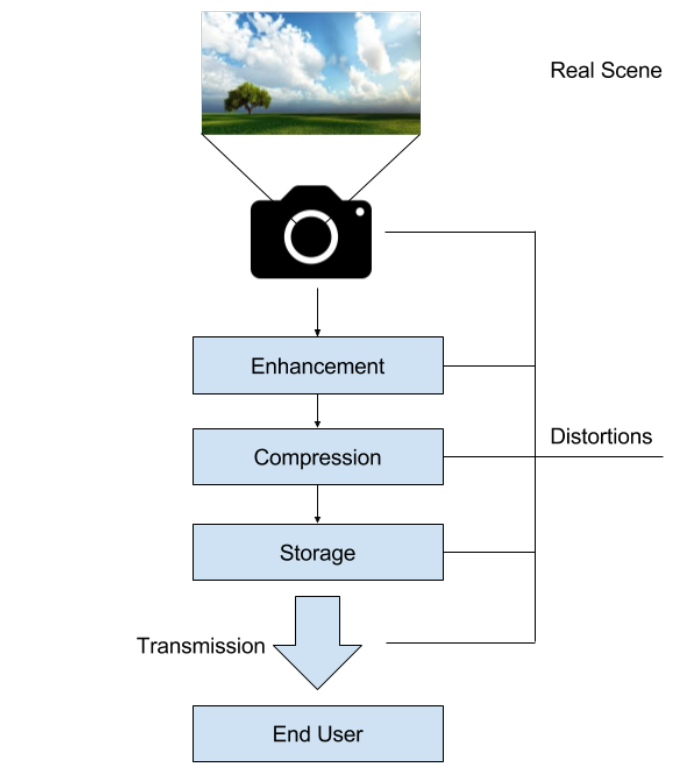
\includegraphics[width=\linewidth]{figures/digitalsteps.png}
  \caption{Digital images suffer from distortions on every step.}
  \label{fig:digimgs}  
\end{figure}
  
End users tend to be more inclined to select a content provider, a service provider, and a display device that can better meet their image quality expectations at delivery. Thus, optimizing these respective technologies to deliver perceptually good results becomes crucial for all content providers, service providers, and display providers, and in order to do so, perceptual image quality needs to be estimated. In addition, in order to determine the perceptual quality, this estimation process should be automated as much as possible to make it independent of the availability of human observers. 

Image Quality Assessment (IQA) aims to measure the perceived quality of the visual signal based on its statistical characteristics and human perceptual mechanism, which is widely required in numerous applications for image processing. IQA plays a vital role in guiding, implementing, optimizing and verifying many visual processing algorithms and systems \cite{Lin2011,Wang2018,Wang2018a,Zhang2016}. 
In particular, image compression is one of IQA's most representative applications, which can be used in the process of optimizing rate distortion to obtain compressed images with better visual quality at the same bit-rate level.  \cite{Channappayya2008,Chen2010,Wang2012,Zhang2017,Zhang2017a,Ma2016}. 
The traditional methods of image compression mainly use the quality metrics based on signal-fidelity, which are less correlated with human perceptual quality , e.g., MAE (mean absolute error), MSE
(mean square error), SNR (signal-to-noise ratio), PSNR (peak
SNR) and their relatives. 
While these metrics have many favorable properties, e.g. clear physical meaning and high calculation efficiency, they severely impede the improvement in compression performance by further reducing image visual redundancies due to their poor consistency with human visual perception. 

Many perceptual quality metrics have been proposed over the past few years to obtain more consistent measures with human visual perception. 
According to the availability of a reference image, these methods can be divided into three categories, i.e., full reference (FR) ones where the pristine
reference image is available, reduced reference (RR) ones
where partial information of the reference image is available
and no reference (NR) ones where the reference image is
unavailable. 
For image compression problem, the reference images are available at the encoder side such that the FR-IQA
algorithms are applicable.

Many FR-IQA based algorithms have been proposed over time. One class of these
algorithms including SSIM \cite{Wang2012}, FSIM \cite{Zhang2011}, RFSIM \cite{Zhang2010} use handcrafted features (attributes (edge, color, etc.) in data (images) that are relevant to the
modeling problem) that supposedly captures relevant factors affecting image quality. 
Although their performance is acceptable, there is still large room for improvement regarding the accuracy with which they reproduce human judgment of quality. 
Another set of algorithms, including convolutional neural network
(CNN) based approaches \cite{Bosse2018,Kang2015}, employ automatic learning of features from the
raw image pixels, which are superior and more efficient as they make feature selection automatic and embedded within the system itself.

\section{Motivation}

Most of the existing IQA
databases usually contain limited distortion levels (5-6 levels)
covering the whole quality range from \enquote{Bad} to \enquote{Excellent},
which make the images in adjacent distortion levels obviously
different and easy to rank. 
To describe the obvious and subtle quality differences between two images, Zhang \textit{et al} \cite{Zhang2019} use
the terms \enquote{coarse-grained} and \enquote{fine-grained}.
More specifically, the images with \enquote{coarse-grained} quality differences correspond to the compressed ones generated using the same codec at obvious different bitrates, while the images with \enquote{fine-grained} quality difference correspond to the compressed ones generated using
different optimization methods at the same bitrate. 
Therefore, these databases with coarse-grained distortion variations
for the same image may not be able to provide sufficient
information to further improve the performance of IQA algorithms in evaluating fine-grained quality differences. 

Another weakness for the existing IQA databases is that
they only contain a few reference images with limited visual content. 
To solve this problem patch-based methods are gradually used in IQA, e.g. CNN-IQA \cite{Kang2014}, CORNIA \cite{Ye2012}
The patch-based learning methods requires the \enquote*{ground truth} of patch quality for training
but there are only the ground truth quality of images instead
of patches in IQA datasets.
To deal with this problem, existing works usually assign the image quality score to all patches
in this image as their \enquote*{ground truth}, e.g. CNN-IQA \cite{Kang2014}. 
This approach might introduce much noise in patches labels because in some distortion types the quality of patches in one
image varies much and the patches quality score can’t be
simply assigned as the image quality core. 

Based on all these observations, this project promotes IQA in the new challenges of fine-grained quality assessment task by constructing a large-scale Image-Patch Quality Assessment database with fine-grained distortion differences. 
We also analyze 7 state-of-the-art IQA algorithms on the proposed database and show that there is still a large room to improve the IQA in the prediction of the fine-grained quality preference. 
Finally, we propose an FR Image-Patch model to help estimate the \enquote*{ground truth} quality of patches based on a state-of-the-art CNN architecture.   
   
\begin{figure}[H]
  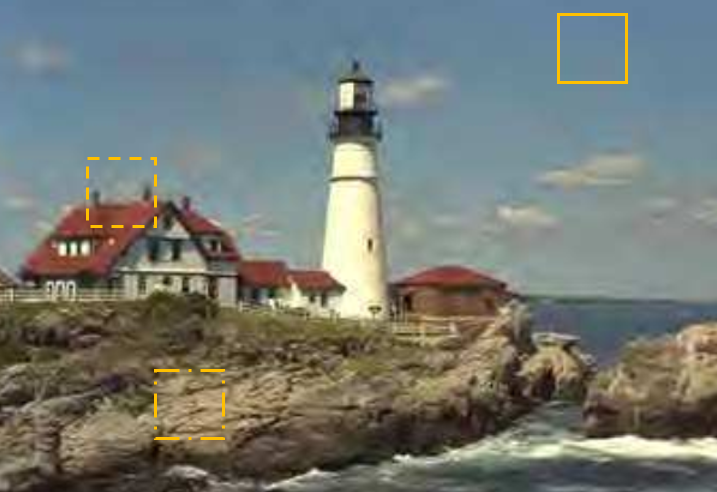
\includegraphics[width=\linewidth]{figures/first.png}
  \caption{Example of JPEG distorted image. Different patches have different qualities.}
  \label{fig:dist-exmaple}
\end{figure}


\section{Contributions}

This thesis provides the following contributions:

1. \textbf{Image-Patch Quality Assessment dataset}

To our knowledge, this dataset is the first one constructing to provide benchmark for compressed image patch quality assessment, and also benefit for perceptual-based image compression. 
The existing databases with coarse-grained quality are inefficient to evaluate IQA algorithms especially patch-based methods on images with fine-grained quality differences. 
In perceptual-based image compression problem, for each coding block there are many coding modes to select a according their rate-distortion costs. Therefore, the proposed dataset can help researchers in image compression community to select the best IQA method to do the perceptual based image optimization. 7 well-know IQA algorithms are evaluated and analyzed on the proposed database to reveal some limitations of the existing algorithms.

2. \textbf{Deep Image-Patch Neural Network Design}

We also investigate different FR methods to model the relationship between the image patch and patch quality score. 
After multiple of experiments, Deep Image-Patch Quality Assessment (DIPQA) is proposed to address the problem in and end-to-end optimization. 
We adapt the concept of Siamese networks know from classification task \cite{BROMLEY2004,Chopra2005} that allow for a join regression of the features extracted from the reference and distorted patch using a deep convolution neural network. 

\section{Thesis Outline}

The rest of this thesis is organized as follows. After this introduction, we present the literature review in Chapter 2 in which we introduce the fields of image quality assessment and deep learning. Next, our methodology is described in Chapter 3. Chapter 4 shows the evaluation of our database and proposed neural network based on experiment result. Finally, the conclusions and future directions are given in Chapter 5.\newpage\cleardoublepage
\chapter{Background}

\section{Image Quality Assessment}

As portrayed in the introduction, image quality assessment (IQA) is vital for many applications, but on the other hand is hard to achieve as such because of its reliance on the quantification of human perception. 
The most solid approach to embrace IQA is through subjective assessments, but this is not practical in real-life applications since users can’t always be dependent upon to comment on the perceived quality. 
On the other hand, objective image quality assessment focuses on implementing human perception models that can estimate the quality of an image as perceived by a person based solely on pixel analysis information.

In the following, we briefly review current subjective quality assessment methods to then go deeper in the state-of-the-art of methods for objective quality assessment.

\subsection{Subjective image quality assessment}

Subjective image quality assessment methods use human observers to express their personal opinion on the quality of images which are used to be assessed. 
Because humans are the end users in a large portion of the multimedia applications, subjective IQA methods are the most reliable and accurate for image quality assessment.

Several international standards have been proposed for performing subjective image quality assessment such as , ITU P913 \cite{ITU2014}, ITU P910 \cite{ITU-TRecommendationP.9102008} and ITU BT 500 \cite{Bt2002}. 
The main objective of subjective IQA methods for a given set of images is to assign a score to each of them that quantifies the perceived quality of the user. In most cases, a scaling process can be achieved, either explicitly or implicitly.

Subjective testing usually focuses on quantifying average observer's perceived quality. 
A group of subjects is requested to evaluate an image and give its perceived quality score.
These scores are then accumulated and the final score is calculated to reflect the quality perceived by an average observer. 
For the calculation of this final score, different scales could be used, for example, direct scaling in which the perceived quality of an image is calculated as the mean of the scores assigned to that image by each subject. (Mean Opinion Score (MOS) or Differential Mean Opinion Score (DMOS)). 
The objective IQA methods (to be followed) are intended to use different models to predict these mean values.

Despite being the most accurate and reliable, subjective IQA methods are highly impractical for real-world applications as it is very expensive and time-consuming to gather an adequate number of observers to evaluate image quality. Consequently, more practical objective IQA methods are used for many applications.

\subsection{Objective image quality assessment}

Rather than using human observers, objective IQA methods are aimed at using relevant models that can predict image visual quality as perceived by humans. Because these algorithms require no human observer, they are fast and very practical for many applications in the real world, such as image enhancement, image restoration, etc.

To estimate the perceptual quality of the given image (called test image), either in the presence or absence of its reference image, most of the objective IQA methods share a common framework of three main phases as illustrated in Fig.\ref{fig:obj-fw}. These
three phases are described in the following

\begin{figure}[H]
  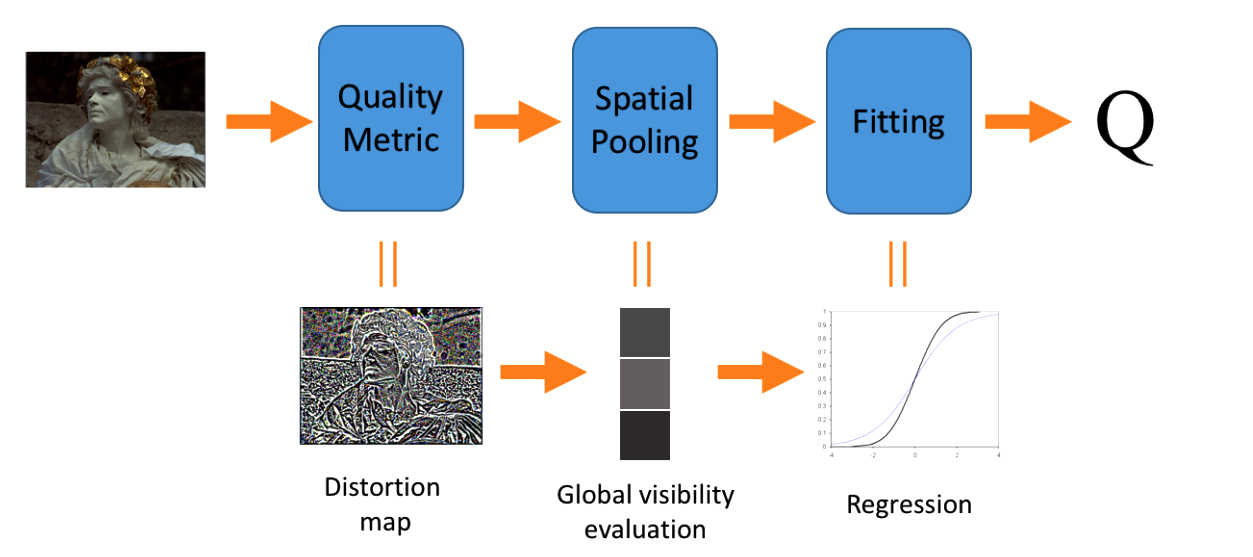
\includegraphics[width=\linewidth]{figures/objective-framework.png}
  \caption{General Objective image quality assessment framework}
  \label{fig:obj-fw}
\end{figure}

1. The test image is processed pixel by pixel or region by region in accordance with the objective IQA method used to measure the amount of distortion present in it. This phase then outputs the distortion measured in the form of a distortion map containing the image quality local description. This step is equivalent to the feature extraction. 

2. A multidimensional phase is produced in the first phase, but humans perceive image quality as a single global entity rather than the local properties of an image. A spatial pooling strategy is generally used to downsample the multidimensional distortion map to a single quality score in order to produce a global quality assessment. \cite{Wang2006}

3. Since in the first two phases non-linearity, which characterizes perception, is not used, the output may not be sufficiently accurate. Thus, to increase the overall accuracy of the framework, an appropriate strategy could be applied. This requires a set of images along with their subjective quality scores (obtained through subjective testing), and a parametric model whose parameters are learned through the analysis of image model predictions and their actual subjective scores through regression. This learned model is then used to transform predicted scores into better estimates allegedly consistent with human perception. 

Objective IQA strategies are classified into three large categories.

\subsubsection{Full-reference image quality assessment (FR-IQA)}

FR-IQA methods aim to achieve objective IQA goals while taking as input both reference and test images. Because these algorithms also require reference images to estimate visual quality, their scope is limited to a few applications where reference images are easily available, such as compression of images and watermarking. 

Over time, a lot of FR-IQA algorithms were proposed. According to one of these methods, image quality can be computed as a peak-signal-to-noise ratio (PSNR), which is simply a ratio of a signal's maximum power and distortion power. The distortion power is generally calculated to calculate the pixel-wise difference between the reference and the distorted image in terms of mean-square-error (MSE). PSNR has the advantages of being simple and very inexpensive computationally, but it does not deliver very good performance because the essential physiological and psychophysical characteristics of the human visual system (HVS) are not included in this algorithm. 

Another FR-IQA algorithm, the Structural Similarity Index (SSIM) \cite{Wang2004}, advances FR-IQA from raw pixels to structures. It is based on the assumption that HVS is highly adapted to extract structural information present in an image, and degradation of images is perceived as a change in this structural information. SSIM therefore aims to evaluate the quality of an image by measuring variations in the structural information of distorted images (in relation to their reference image). In evaluating the perceptual quality of images, SSIM has been shown to outperform PSNR 

Another lately proposed FR-IQA \cite{Zhang2011} algorithm is the Function Similarity Index (FSIM). It is based on the fact that HVS uses low-level features to understand images (like edges and zero crossing). FSIM uses two features to estimate an image's quality: a primary feature called Phase Congruency, which is a contrast-invariant dimensionless measure of the local structure's significance, and an image gradient magnitude feature. FSIM shows superior performance on different datasets than PSNR and SSIM algorithms. 

Recently, Bosse \emph{et al.} \cite{Bosse2018} presents an IQA data-driven approach based on deep neural networks. The network consists of 10 convolution layers and 5 pooling layers for extraction of features, and 2 fully connected layers for regression, making it significantly deeper than related IQA models. Unique features of the proposed architecture are that I it can be used in a no-reference (NR) as well as in a FR-IQA setting with slight adaptations and (ii) it enables joint learning of local quality and local weights in a unified framework, i.e. the relative importance of local quality to the global quality estimate. 

\subsubsection{Reduced-reference image quality assessment (RR-IQA)}

RR-IQA methods aim to achieve objective IQA goals by estimating the quality of the test image while using partial reference image information. Usually this partial information is in the form of features extracted from the images of the reference. 

In communication networks, RR-IQA finds its application that is used to transmit images and videos. Using RR-IQA algorithms, partial reference image information transmitted through these communication networks can be used to track visual quality degradation of images and videos transmitted. In similar applications, therefore, RR-IQA algorithms are preferred over FR-IQA algorithms as presented in \cite{Atsawaraungsuk2015, Redi2010}.

\subsubsection{No-reference image quality assessment (NR-IQA)}

NR-IQA methods are intended to achieve the objectives of objective IQA by using only test images to estimate the quality of the image. Due to the lack of information on reference images, these methods are considerably more challenging than FR-IQA and RR-IQA. But due to their application in the wide variety of fields, they are also more desirable, ranging from image processing to image enhancement, where reference images are usually not available. NR-IQA methods are also used in a wide range of online applications, such as communication systems, image acquisition systems, etc. \cite{Chandler2013}, making it very important for them to be computationally cheap. 

Some early NR-IQA attempts used distortion-specific methods that approach IQA tasks by using models very specific to a specific type of distortion. These methods are more specific to applications where there is prior knowledge of the type of distortion. For example, in an application to measure quality losses in compressed images, knowledge of the appearance of compression artifacts, such as blocking and ringing, could be used to design NR-IQA methods that can detect their visibility 

It is more useful to have algorithms, regardless of the types of distortion, that can be applied for general purpose NR-IQA. Existing NR-IQA approaches for general purposes could be further divided into two broad categories: Natural scene statistic based approaches (NSS) and Feature learning based approaches


\subsection{IQA in Visual Data Compression}

\begin{figure}[H]
  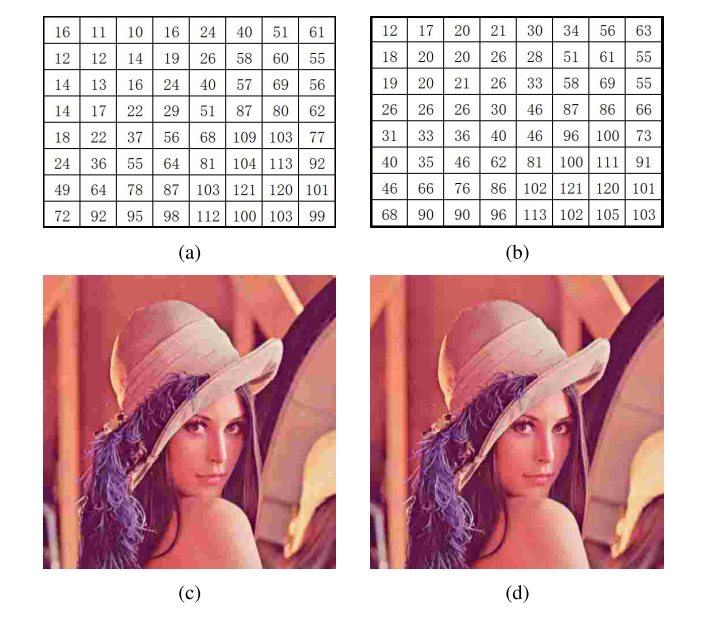
\includegraphics[width=\linewidth]{figures/jpeg.png}
  \captionsetup{justification=raggedright}
  \caption{Examples of quantization table and the corresponding compressed
JPEG images.} 
  \label{fig:jpeg}
  \subcaption*{(a) JPEG default quantization table at quality factor equal to
50; 
    \newline(b) Optimized quantization table with the optimization goal of MS-SSIM; \newline(c) JPEG image using default quantization table at QF = 10, 0.234 bbp,
PSNR = 30.45, SSIM = 0.819, MS-SSIM = 0.946; \newline(d) JPEG image using
MS-SSIM optimized quantization table, 0.226 bpp, PSNR = 30.49, SSIM = 0.818, MS-SSIM = 0.953}

\end{figure}

While the bitstream has been normalized by image coding standards, different coding parameters or modes determined by different IQA metrics will obviously result in distinct compression performance. In JPEG, the custom quantization table is one of the optional coding parameters, and the default table is empirically determined based on human perception \cite{Wallace1992}. For example, in Fig.\ref{fig:jpeg}(a), which is scaled to generate quantization tables for other quality factors, the quality factor (QF) quantization table of the luminance component equal to 50 is shown. In addition to the standard JPEG quantization table, the open source and well-optimized JPEG codec, \emph{libjpeg}, has adopted another 8 quantization tables, one of which is an optimized MS-SSIM-based quantization table as shown in Fig.\ref{fig:jpeg}(b). 

In \cite{Ratnakar2000}, the researchers proposed optimization of the image-dependent quantization table based on the signal fidelity-based metric, MSE, which achieved substantial bit rate savings at the same quality as PSNR. However, because of the poor correlation between perceptual quality and PSNR, these optimization strategies can not ensure the same visual quality improvement. The researchers introduced SSIM and its variants into image and video coding in \cite{Channappayya2008}, \cite{Wang2012} and \cite{Ou2011} to optimize the process of rate distortion, but the performance improvement is not yet so satisfying. The upper and lower boundaries of the average SSIM index were derived for the first time by Channappayya \emph{et al.}\cite{Channappayya2008} as a function of the quantization rate for different source distributions, e.g. uniform, Gaussian and Laplacian. Wang \emph{et al.}\cite{Wang2012} used SSIM as the quality metric for optimizing rate distortion instead of MSE and achieved a bit rate saving of about 5\%-10\% compared to the original H.264/AVC. Ou \emph{et al.} \cite{Ou2011} applied SSIM to the problem of perceptual rate control with a gain of 0.008 SSIM (corresponding to a saving of 14\ percent bitrate). We can see from this work that the improvements in quality are still small. 

Essentially, with regard to the compression of the perceptual image, although different encoding optimization strategies can improve the image quality at the same bit rate level, the quality fluctuations are usually limited within a small range. However, most traditional IQA databases contain only coarse-grained compression distortion levels, and IQA algorithms on the fine-grained quality prediction for image compression problem can not be evaluated well. For example, the scaled quantization tables in Fig.\ref{fig:jpeg}(a) and \ref{fig:jpeg}(b), respectively, compress the JPEG images in Fig.\ref{fig:jpeg}(c) and \ref{fig:jpeg}(d) at similar bitrates. Although the image shows less blocking artifacts in Fig.\ref{fig:jpeg}(d), it has a lower SSIM value but higher PSNR and MS-SSIM values than the image shown in Fig.\ref{fig:jpeg}(c). These different IQA algorithms show opposite quality rankings on the level of fine-grained distortion, which motivates us to re-examine existing IQA algorithms and examine their suitability to distinguish fine-grained distortions 

\section{Neural Networks}

\subsection{Artificial Neural Network}

Artificial Neural Network (ANN) is not a brand new idea. It was first introduced as a computational model of "nerve net" in the human brain by Warren McCulloch and Walter Pitts[17] in 1943. After that, the concept and architecture of neural networks are further developed by follow-up researchers. Neural networks have long been constrained by hardware performance. The advancement in GPU design and brain science led to a boom in the development of neural networks only in recent decades. 

\begin{figure}[H]
  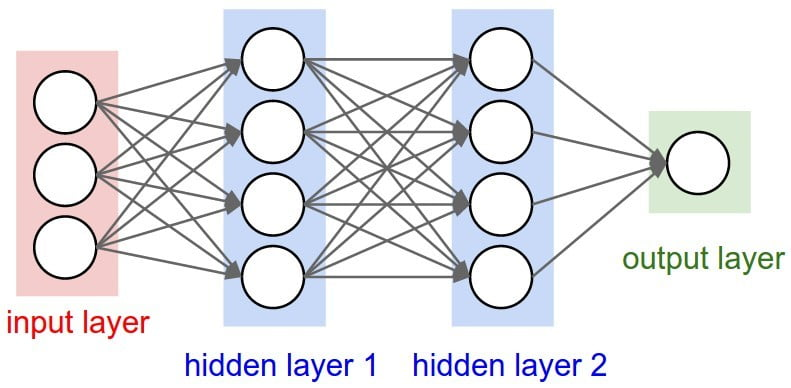
\includegraphics[width=\linewidth]{figures/ann.jpg}
  \caption{The basic structure of Neural Network.}
  \label{fig:ann}
\end{figure}

A common modern neural networks consist of a large number of nodes called neurons. Each neuron does a simple calculation, usually $y = Wx + b$, where $W$ is called Weight and $b$ is called Bias. The neurons form multiple layers and the result value $y$ of each neuron is then passed to the neurons in the next layer. The first layer is called input layer as shown in Fig.\ref{fig:ann}. As its name implies, it takes features from outside the network as input. The last layer is output layer and its output value is the prediction given by the neural network.

\subsection{Training Neural Network}

First, Weight Metric and Bias Metric are initialized with random values (or pre-trained value obtained from other benchmark data). A training of the neural networks is required to adjust those parameters to fit into a particular task.

The most common and popular method of training neural network is back-propagation (BP). The goal of back-propagation is to compute the partial derivative, or gradient, $\frac{\partial E}{\partial w}$ of a loss function E with respect to any weight w in the network. The loss function
$E$ calculates the difference between prediction of neural network and its expected output, after one or a batch of sample data go through the network. A loss function is usually defined as:

\begin{equation} \label{eq:lossabs}
E=\frac{1}{N}\sum_{i=1}^{N}|f(x_i)-y_i| 
\end{equation}

or

\begin{equation} \label{eq:losssqr}
E=\frac{1}{N}\sum_{i=1}^{N}(f(x_i)-y_i)^{2} 
\end{equation}

where $f(x)$ is the equivalent function fo the neural network. Equation \ref{eq:lossabs} is called $L1$ loss while equation \ref{eq:losssqr} is called $L2$ loss. In practice, $L2$ loss is the most popular one because it is more sensitive to examples that far away from expected output. Thus
the trained neural network is hopefully more general. On the other hand, $L1$ loss is not
that sensitive to a minority of output that far from the expectation and takes care of the
average error of the majority. It is especially useful when training data is not very carefully
collected and may contain incorrect samples.

Thus the progress of training by BP can be presented as:

\begin{enumerate}
  \item Put one batch of training data through the neural network
  \item Calculate the loss between output and ground truth
  \item Go backward the network and calculate the partial derivative, or gradient, $\frac{\partial E}{\partial w}$
of loss function $E$ with respect to each weight $w$ in the network
  \item Update the weights in the network according to loss, gradient and learning rate (LR)
  \item Repeat step 1 to 4 until training ends, usually when a certain number of cycles set
by researcher is reached or the loss value is smaller than a threshold
\end{enumerate}

This method is called \enquote{back-propagation} partly because the partial derivative is calculated using chain rule:

\begin{equation}
\frac{\partial E}{\partial w_{ij}} = \frac{\partial E}{\partial o_j} \frac{\partial o_j}{\partial net_j} \frac{\partial net_j}{\partial w_{ij}}
\end{equation}

where $E$ is the loss function, $w_{ij}$ is the weight from neuron $i$ to neuron $j$, $o_j$ is the output of the neuron $j$, $net_j$ is the weighted sum of outputs to neuron $j$ from the previous layer.

We can calculate them one by one from the output layer to input layer and use the result in later layers for calculating the former layers. Therefore, calculating partial derivative is actually quite cheap when doing backward.

A neural network with multiple layer structure has proved its power on image recognition. However, it suffers from \enquote{the curse of dimensionality} heavily. It means that the number of parameters in the network goes up quickly when the dimension (resolution) of input image increases. Early neural networks work on low resolution images such as $20 \time 20$ and $32 \time 32$. Early benchmark datasets, MNIST and CIFAR10 for instance, are also collections of small images with $20 \time 20$ and $32 \time 32$ pixels. At that time, neural networks can take care of those images with hundreds or thousands of parameters. When the size of target image rise to around $200 \time 200$, an input layer with 40000 neurons is needed. Assuming the first hidden layer is fully connected and has the same number of neurons as the input layer, which is quite common in practice, at least $40000 \time 40000$ individual parameters is needed in just 2 layers. The mass of parameters not only consumes computing resources, but also causes serious overfitting problems. 

Overfitting means that a statistical model tries to describe each training sample rather than to find out regular patterns among the sample collection. Fig.\ref{fig:overfit} shows a simple case of overfitting. The regression function tends to "remember" the distinguishing features of each sample individually but fails to figure out the trend of all samples. Although it passes every sample point and has 0 loss, it is not generalizable to unseen data. Even a linear function has more prediction power than it. 

\begin{figure}[H]
  \centering
  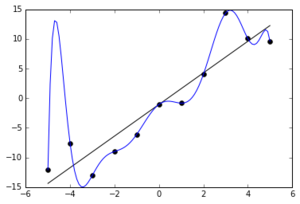
\includegraphics[width=.7\linewidth]{figures/overfit.png}
  \caption{The function overfit the train samples.}
  \label{fig:overfit}
\end{figure}

Overfitting usually happens when neural network has too many parameters compared to the number of training samples, which enables the network easily remembering all samples. To limit the number of parameters in neural network, researchers find a way to reuse parameters in different parts of the image, which is a Convolutional Neural Network (CNN)

\subsection{Convolutional Neural Network}

A CNN is one type of neural network that specially designed for image recognizing. The architecture of CNN comes from the organization of animal visual cortex. Fig.\ref{fig:cnn} shows the basic structure of a convolutional neural network. $X_{i,j}$ represents the pixels in the input image. A is the kernel of the first convolutional layer and is repeatedly used on each block of four pixels. The neurons on the second layer then takes the outputs of the first layer as their inputs and use the same kernel B. Fig.\ref{fig:kernel} shows the mapping between 2 layers. One blocked in the front layer, which is a  $m \times n \times d_1$ tensor ($m = n$ in most cases), is multiplied by a $m \times n \times d_1 \times d_2$ kernel and mapped to a $1 \times 1 \times d_2$ block in the next layer. The $m \times n \times d_1$ block in the front layer is called receptive field, which means all neurons in such block is connected to one neuron in the next layer, and their information is gathered together by a neuron in next layer.

\begin{figure}[H]
  \centering
  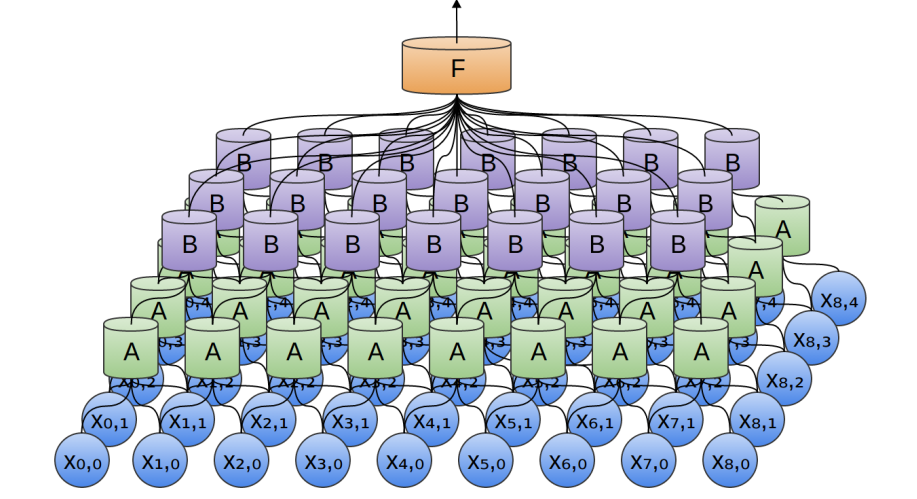
\includegraphics[width=\linewidth]{figures/cnn.png}
  \caption{CNN share the kernel on each layer.}
  \label{fig:cnn}
  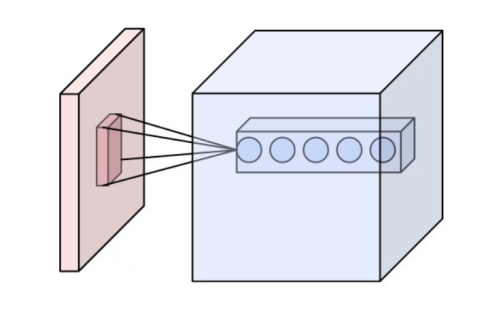
\includegraphics[width=0.5\linewidth]{figures/kernel.png}
  \caption{Kernel that maps $m \times n \times d_1$ block in the previous layer to an $1 \times 1 \times d_2$ block in next layer.}
  \label{fig:kernel}
\end{figure}

CNN is proved to be very efficient in pattern recognition and other image classification tasks. Its superior performance comes from some particular features. The most important feature is perhaps its spatial invariant. Since the same kernel is used repeatedly in the whole input space, it can detect its corresponding pattern no matter where the pattern shows up. This feature significantly reduces the number of patterns the network needs to learn. 

Another important feature is its ability of abstracting and concentrating information. In Fig.\ref{fig:cnn}, each neuron $A$ (instance of kernel) on first layer accesses information from 4 pixels. On the second layer, each neuron $B$ connect to 4 neurons in the first layer, which means it can access information gathered from 9 pixels in the input image. As the network goes deeper, the neurons in later layers get access to larger area of the input image. At last, at the final layer, the network gets an overall abstract sense of the input image. All of these concentration and abstract procedure are learned automatically by back-propagation. It is still a mystery to researches that how those things exactly happen because the mid product of hidden layers are really difficult to understand by human beings.

\textbf{ReLU Layers} 

ReLU layers usually stand between 2 convolutional layers. ReLU stands for Rectified Linear Units. ReLU layer applies the non-saturating activation function to the outputs of convolutional layers:

\begin{equation} \label{eq:relu}
f(x) = max(0,x)
\end{equation}

ReLU layers are very simple but they efficiently add nonlinear properties to the decision
making function of the overall network as well as the sigmoid function:

\begin{equation} \label{eq:sigmoid}
f(x) = \frac{1}{1+e^{-x}}
\end{equation}

and the hyperbolic tangent function:

\begin{equation} \label{eq:hypo}
f(x) = \tanh(x)
\end{equation}

\begin{figure}[H]
  \centering
  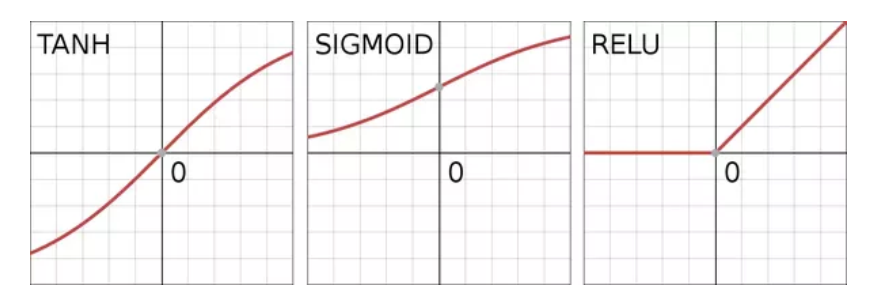
\includegraphics[width=\linewidth]{figures/activation.png}
  \caption{Common nonlinear functions used in CNN: ReLU, Sigmoid and hyperbolic tangent.}
  \label{fig:activation}
\end{figure}

Fig.\ref{fig:activation} shows the response of 3 methods. The 3 methods share the same idea of inhibiting negative outputs and amplifying/keeping positive outputs of the early layers, which is a simulation of how human brain cells work. Hyperbolic tangent function and sigmoid function are widely used in old models but ReLU function becomes more preferable recently because it is proved to be much computational cheaper without making any significant differences in accuracy

\textbf{Pooling Layers} 

\enquote{Pooling} is a nonlinear down-sampling method widely used in CNNs. Fig.\ref{fig:pool} shows a common max pooling layer with a $2 \times 2$ filter size and a stride of 2. The filter move through the entries with a certain stride, pooling layer maps each block in former layer to a single value. Pooling layer concentrates the information in former layer and provides the later layers a larger \enquote{vision} in the original image. Also, pooling helps reducing the number of parameters in the network and hence has an effect of overfit control. The most popular pooling methods are max pooling and min pooling, where the filter takes the max or min value in each block as the output. Average pooling, which uses the average of all values in the block as output is also commonly used in old days. However, it has given its place to max pooling since the later one is proved to work better in practice.

\begin{figure}[H]
  \centering
  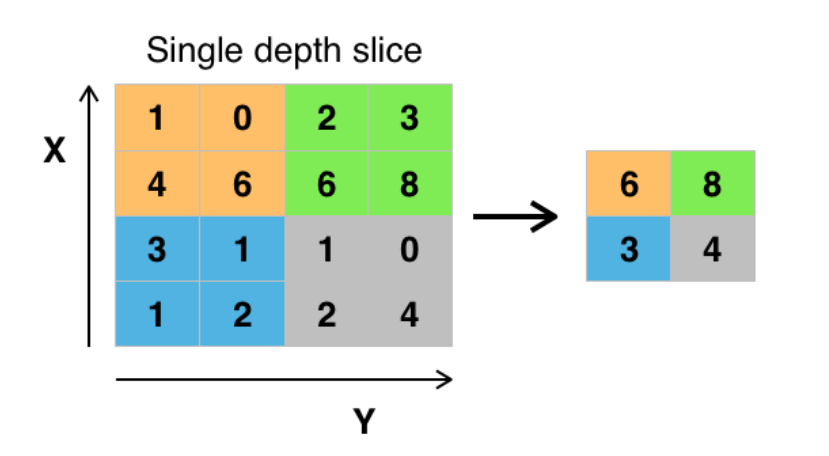
\includegraphics[width=\linewidth]{figures/pooling.png}
  \caption{A max pooling layer with a $2 \times 2$ filter size and a stride of 2}
  \label{fig:pool}
\end{figure}\newpage\cleardoublepage
\chapter{Methodology}

\section{Database Construction}

All available image quality benchmark databases are only suitable for evaluating the quality of images as a whole and not able to investigate which parts of the testing image contribute to the testing results or the score for a particular patch of image. 
In this project, we set up an experimental database to evaluate the quality that human perceive for each image patch.

\subsection{Testing image database}

A good database for testing is critical to be the success of the research. 
Due to the research orientation for video encoding, testing images are cropped from extracted frames in the video test sequence and noise types are added to the original video by H265/HEVC compression before extracting. 
In this database, we randomly select several patches from each image so that the database includes at least three attributes: smooth texture, complex texture and edge texture.

\begin{figure}[H]
  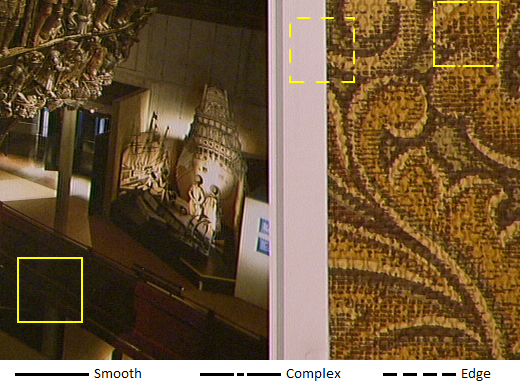
\includegraphics[width=\linewidth]{figures/imgpatches.png}
  \caption{Selected image patch.}
  \label{fig:selected-patch}
\end{figure}

\subsection{Database creation}

There are 40 original source videos of high-definition (1280x720) and full high-definition (1920x1080) being compressed by H.265/HEVC with different Quantization parameters (QPs) with the range from 2 to 50. Testing images are extracted from those testing video sequences. For each video sequence, we select a different number of frames depend on the original video, this number drops in the values from 5 to 15. After that, we select random positions of the image to crop different 128x128 patches of each pair of image. We also crop the center 64x64 patches from the original pair 128x128 to evaluate in the experiments. Finally, we obtain 161,144 images: 40286 pairs of 64x64 patches and 40286 pairs of 128x128 patches.


\begin{table}[H]
  \centering
  \begin{tabular}{| c | c | c | c | c | c | c | c |}
    \hline                          & \multicolumn{7}{c|}{QP} \\ \cline{2-8} 
    \multirow{-2}{*}{Orignal} & 25    & 30   & 35   & 40   & 45   & 50   & 55   \\ \hline 
    &&&&&&&\\
    
\includegraphics[height=1cm]{figures/11.png}                                                 &      &      & 
\includegraphics[height=1cm]{figures/12.png}       & 
\includegraphics[height=1cm]{figures/13.png}       & 
\includegraphics[height=1cm]{figures/14.png}    & 
\includegraphics[height=1cm]{figures/15.png}    & 
\includegraphics[height=1cm]{figures/16.png}    \\ 
    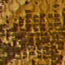
\includegraphics[height=1cm]{figures/21.png}                                                  &       &      &  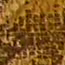
\includegraphics[height=1cm]{figures/22.png}     &  
\includegraphics[height=1cm]{figures/23.png}     &  
\includegraphics[height=1cm]{figures/24.png}     &  
\includegraphics[height=1cm]{figures/25.png}     &  
\includegraphics[height=1cm]{figures/26.png}     \\ 
    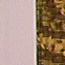
\includegraphics[height=1cm]{figures/31.png}                                                  & 
\includegraphics[height=1cm]{figures/32.png}     & 
\includegraphics[height=1cm]{figures/33.png}    & 
\includegraphics[height=1cm]{figures/34.png}    & 
\includegraphics[height=1cm]{figures/35.png}    & 
\includegraphics[height=1cm]{figures/36.png}    &      &      \\ \hline
  \end{tabular}
  \caption{Example of testing image database.}
  \label{tab:exid}
\end{table}

\subsection{Testing methodology}

Depending on the nature of the test, observers may be expert or non-expert. Studies have found that systematic differences can occur between different laboratories conducting similar tests \cite{Bt2002}. One of the reasons for this is that expert observers have different view in compare with no-experts. Other explanations may include gender, age, and occupation. However, in reality, the majority of consumers should be non-expert observers are chosen for this experiment. Before final selection, all candidates have been checked to ensure that they possess normal visual acuity.

For the purpose of this experiment, 1200 subjects who are undergraduates, graduates, researchers, and lecturers of University of Fire Fighting and Prevention are employed. These subjects have been trained and practiced quality assessment of several sample images.

For the purpose of subject testing methodology, the International Telecommunication Union set the ITU-R BT.500-11 \cite{Bt2002} standard. In such standard, there are several popular subjective methodologies for testing such as Single stimulus categorical rating, Double stimulus categorical rating, Ordering by force-choice pairwise comparison and Pairwise similarity judgments. Double stimulus categorical rating is chosen in this practical. In this method, both the test and reference images are displayed for a fixed amount of time. After that, the images disappear from the screen and observers are asked to rate the quality of the test image according to the abstract scale containing one of the five categories: excellent, good, fair, poor or bad. All those images are displayed randomly. At the beginning of each session, an explanation is given to the observers about the type of assessment, the grading scale, the sequence and timing (reference image, grey, test image, voting period).

The previous image quality assessment methods are only suitable for assess quality of image as a whole. It cannot be directly applied for our testing experiments. Therefore, we modify this image selection method in the standard so that the users can only concentrate and assess the local image patch instead of the whole image. Each pair quality is assessed with the following procedure: The subjects observe the original image within the time T1 at minimum 5s then click on the observing image patch to observe the compressed image within the time T2. After watching at least twice per image, the observers would score on scale of 5 as in Fig.\ref{fig:testing-software}.

\begin{figure}[H]
  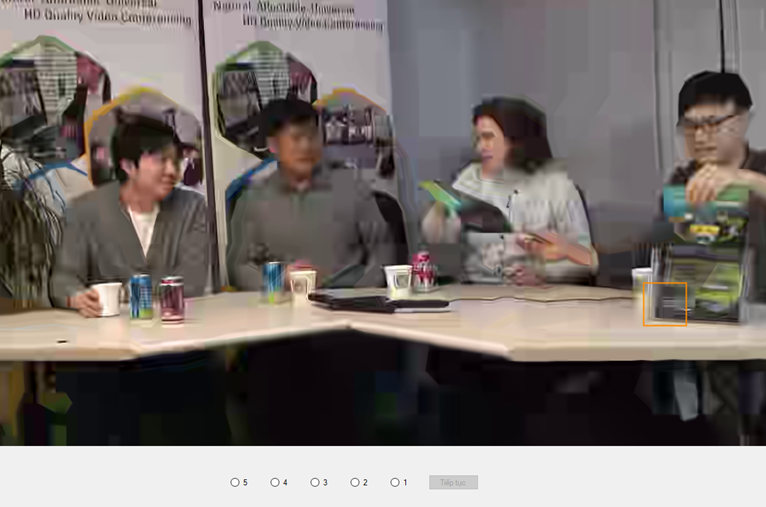
\includegraphics[width=\linewidth]{figures/softtest.png}
  \caption{Testing software screenshot.}
  \label{fig:testing-software}
\end{figure}

At the end of experiment, each pair is scored by the mean of the DMOS that up to 20 subjects give during the experiment.

We carefully select 1511 pairs which are scored by at least 10 people and name this sub-database HMII (Human Machine Interaction Image). HMII is used to evaluate well-known IQA algorithms and our methods in the second contribution. 

\subsection{Benchmark Analyses}

To analyze the efficiency of IQA algorithms, we apply 7 state-of-the-art full reference image quality assessment
methods on the proposed HMII database, to investigate
their performance and demonstrate the new challenges in
fine-grained image-patch quality assessment problem. The FR-IQA algorithms include PSNR, SSIM \cite{Wang2004}, RFSIM \cite{Zhang2010}, FSIM \cite{Zhang2011}, SRSIM \cite{Zhang2012}, UQI \cite{Wang2002}, VSI \cite{Zhang2014}. The implementations of all algorithms are obtained from the public websites. 

\section{Deep Image-Patch Quality Assessment}

\subsection{Architecture}

Being known as a designed architecture to learn the similarity relations between two given inputs, Siamese network has been applied for face verification \cite{Chopra2005} and signature \cite{BROMLEY2004} tasks. The main concept is processing two networks that share the same architecture and weights parallel. In this work, we employ Siamese network for feature extraction. Before feeding the extracted features as input to the regression layers, feature extraction is followed by a feature fusion step. The proposed architecture of DIPQA is sketched in Fig.\ref{fig:dipqa-architecture}

\begin{figure}[H]
  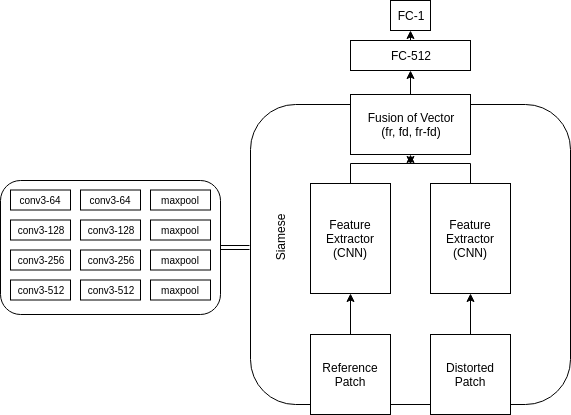
\includegraphics[width=\linewidth]{figures/dipqa.png}
  \caption{Deep Image-Patch Quality Assessment Network Architecture.}
  \label{fig:dipqa-architecture}
\end{figure}

With the successful adaptation for various computer vision tasks \cite{Girshick2015, Shelhamer2017}, especially in image quality assessment \cite{Bosse2018}, VGGnet \cite{Simonyan2014} was chosen as a base network for the feature extraction. The input of the VGG network is the size of 224 x 224 pixels. For the purpose of adjusting the network for 64 x 64 and 128 x 128 pixels, we have tried to change the architecture of VGG network such as: extend the network by 3 layers \cite{Bosse2018}, cut last 3 layers, last 6 layers or even replace VGG with Resnet. Finally, we choose to cut the last 3 layers of VGGnet and achieve the best performance comparing to the other approaches. Our VGGnet-inspired DCNN comprised 12 weight layers as a feature extraction module and a regression module. The features are extracted in a series of conv3-64, conv3-64, maxpool, conv3-128, conv3-128, maxpool, conv3-256, conv3-256, maxpool, conv3-512, conv3-512, maxpool, layers. The fused features are regressed by a sequence of two fully connected layers (FC-512, FC-1). This results in about 17.3 million trainable network parameters. All convolutional layers apply 3x3 pixel-size convolution kernels and are activated through a rectified linear unit (ReLu) \cite{Nair2010} activation function after being normalized with batch normalization. All max-pool layers have 2 x 2 pixel-sized kernels. In order to prevent overfitting, dropout regularization \cite{Sutskever2014} is applied to the fully connected layers with a ratio of 0.5.  

\subsection{Feature Fusion}

The feature extraction layers extract $f_r$ and $f_d$ which are the feature vectors of reference and distorted patch respectively. The regression layers require the network to combine these two vectors in a feature fusion step. A simplest strategy is concatenating $f_r$ and $f_d$ to an unique vector $(f_r,f_d)$. Beside, $f_r-f_d$ is known as a meaningful representation for distance in feature space. Therefore, concatenating $f_r-f_d$ is expected to contribute to learning to relations between reference and distorted patch. The final output of this state is $(f_r,f_d,f_r-f_d)$

\subsection{Training Method}

For better convergence of the optimization, the feature extraction parameters are initialized with VGG13-batchnorm weights which is trained on ImageNet dataset. Our network is trained end-to-end by backpropagation, over a number of epochs. The adaptive moment estimation optimizer (ADAM) \cite{Kingma2015} is employed to alter the regular stochastic gradient descent method. Parameters of ADAM are chosen as recommended in \cite{Kingma2015} $\beta_1 = 0.9, \beta_2 = 0.999, \epsilon = 10^{-8}$ and the learning rate $\alpha$ is initially set to $5\times10^{-4}$. The mean loss, PCC, SRCC over images during validation is computed in evaluation mode after each epoch.\newpage\cleardoublepage
\chapter{Evaluation}

\section{Evaluation Method} 

 
\textbf{Dataset:} 
This database comprises 1511 quality annotated images based on 1511 source reference image patches that are subject to different distortion levels of compression. 
Differential mean opinion score (DMOS) for this dataset were computed for each pair, which is in the range 1 to 5.

\textbf{Evaluation Metrics:}
To evaluate the performances of the IQA algorithms, we used two standard measures, i.e., Spearman's rank order correlation coefficient (SRCC) and Pearson's linear correlation coefficient (PLCC).

\textbf{Experiment Setup:}
Both the experiments in this thesis are performed on HMII database.

For the first experiment, the purpose is to evaluate how well an objective metric agrees with subjective preferences of subjects. We carefully select the Mathlab implementations of 7 algorithms to predict object scores for the entire database. 

For the second one, different models are competed to find the best \enquote*{ground truth} predictor for patch quality. 
Results reported are based on the average performance of 10 folds cross-validation. Deep learning models converge after 50 epochs.   


\section{Experiment results}

\subsection{HMII Benchmark Analysis}

First, we evaluate the pairwise preference consistency using the classic correlation coefficients SRCC and PLCC,
as shown in Table \ref{tab:algos}. 
The SRCC and PLCC are
the average values for the distorted images of the same
reference image, and the top 2 correlation coefficient values are highlighted. 
We can see that the PSNR and UQI are poorly correlated
with human perceptual quality, and even contrary to subjective
results. This defective performance of PSNR is also mentioned in the work of Zhang \emph{et al.}\cite{Zhang2019} about Fine-Grained Quality Assessment. Although VSI combine the HVS features and achieve more
consistent results than PSNR in global image assessment, it is poorly correlated with human perceptual quality in fine-grained patch quality assessment.
For the two correlation coefficients, these IQA methods
shows quite similar characteristics. As a whole, FSIM achieves top 2 performance for all the cases and the SSIM achieves better performance with PLCC while SRSIM performs better with SRCC. 

\begin{table}[ht]
  \centering
  \begin{tabular}{|l|cc|cc|}
    \hline
    \multirow{2}{*}{} & \multicolumn{2}{c|}{ HMII (64x64) }      & \multicolumn{2}{c|}{ HMII (128x128) }    \\ \cline{2-5} 
    & PLCC           & SRCC           & PLCC           & SRCC           \\ \hline
    SSIM\cite{Wang2004}             & \textbf{0.785} & 0.787          & \textbf{0.795} & 0.797          \\
    RFSIM\cite{Zhang2010}             & 0.774          & 0.757          & 0.789          & 0.759          \\
    FSIM\cite{Zhang2011}              & \textbf{0.794} & \textbf{0.799} & \textbf{0.824} & \textbf{0.815} \\
    PSNR              & 0.200          & 0.737          & 0.194          & 0.752          \\
    UQI\cite{Wang2002}               & 0.023          & 0.621          & 0.012          & 0.589          \\
    VSI\cite{Zhang2014}               & 0.765          & 0.765          & 0.768          & 0.786          \\
    SRSIM\cite{Zhang2012}             & 0.777          & \textbf{0.803} & 0.718          & \textbf{0.803} \\ \hline
  \end{tabular}
  \caption{PLCC and SRCC for different IQA algorithms}
  \label{tab:algos}
\end{table}

In addition to visualize the objective score by the top 3 IQA algorithms, we plot the distributions of subjective scores and objective scores on a 2-D graph and also plot the fitted curve on the same figure. The following figure shows the scatter distributions of subjective DMOS versus the predicted scores obtained by the SSIM, FSIM and SRSIM on the proposed database.


\begin{figure}[H]
  \centering
  \begin{subfigure}[b]{0.5\textwidth}
    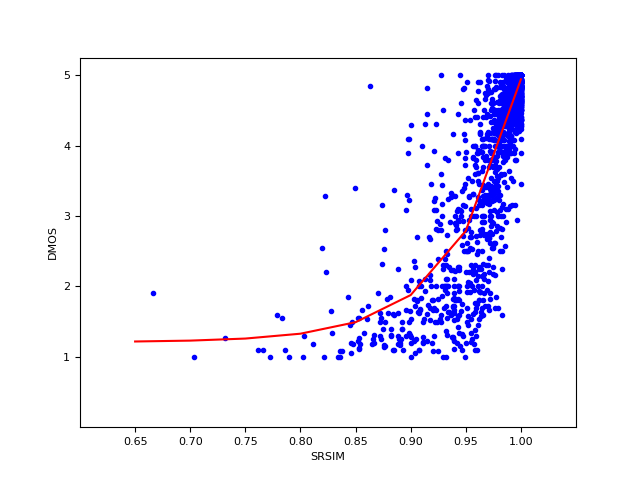
\includegraphics[width=\textwidth]{figures/srsim.png}
    \caption{SRSIM}
    \label{fig:srsim}
  \end{subfigure}%
  ~ %add desired spacing between images, e. g. ~, \quad, \qquad etc.
  %(or a blank line to force the subfigure onto a new line)
  \begin{subfigure}[b]{0.5\textwidth}
    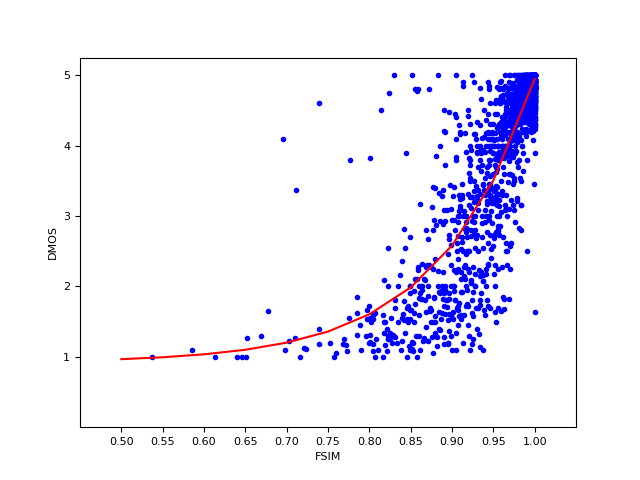
\includegraphics[width=\textwidth]{figures/fsim.png}
    \caption{FSIM}
    \label{fig:fsim}
  \end{subfigure}
  ~ %add desired spacing between images, e. g. ~, \quad, \qquad etc.
  %(or a blank line to force the subfigure onto a new line)
  \begin{subfigure}[b]{0.5\textwidth}
    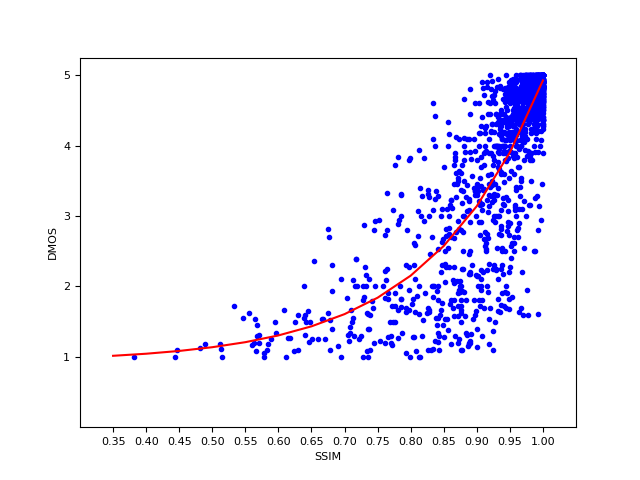
\includegraphics[width=\textwidth]{figures/ssim.png}
    \caption{SSIM}
    \label{fig:ssim}
  \end{subfigure}
  \caption{Objective Score by top 3 IQA on HMII}\label{fig:animals}
\end{figure}

From the plots, we can see that these IQA algorithms tend to predict higher score for patches. 
SRSIM and FSIM frequently predict score which is higher than $0.9_{[0-1]}$ for the image with DMOS is greater than $2_{[1-5]}$.
Although FSIM achieves highest performance with the two correlation coefficients, SSIM achieves more consistent results with subjective results on the diagrams.
These
results prove that some existing IQA models perform poorly
in distinguishing the fine-grained distortion levels, which are
feasible to determine by human visual system. Therefore, these
metrics may not be suitable for perceptual-based image compression because the distortion differences between various
coding modes are usually marginal. Moreover, the fine-grained
image-patch quality assessment is demanded and should be evaluated
on the HMII databases.

\subsection{Image-Patch Models}

In this experiment, we use the following models to evaluate with our proposed DIPQA:

\begin{itemize}
  \item \textit{IPM}: Zhang \textit{et al.}\cite{Zhang2019} assume the the curve model to predict image-patch quality is a cubic polynomial function:
  $$f(\Phi(\textbf{d});\theta) = a\Phi(\textbf{d})^{3} + b\Phi(\textbf{d})^{2} + c\Phi(\textbf{d}) + d$$
  where $\theta = {a, b, c, d}$ are the parameters for the non-linear function of Image-Patch model and $\Phi(\textbf{d})$ represents the feature of patch $\textbf{d}$. MSE and SSIM are chosen for the design of features. In our work, we tried top 3 FR-IQA methods from the first experiment: SSIM, FSIM and SRSIM.  
  
  \item \textit{DIQaM}: Bosse \textit{et al.}\cite{Bosse2018} present a Deep Neural Networks for No-Reference and Full-Reference Image Quality Assessment which obtains superior performance on different IQA benchmarks. We utilize the extractor architecture from this paper to train a Deep Neural Network on our database.
\end{itemize}

First, we use the previous works to extract the SSIM, FSIM and SRSIM feature for IPM. Then, the above curve model is fitted using the least square method to obtain the parameters that best fit the learning set. DIQaM, DIPQA (VGG extractor) and DIPQA (VGG finetuning) is built with the similar architecture which share them same regression part. With the proposed DIPQA, we approach with two different tuning strategies: one is fine-tuned with the VGGNet weight and then retrained with HMII; the other one use VGGNet as a feature extractor, this part is not trained with the entire network.
  
% Second contribution
\begin{table}[ht]
  \centering
  \begin{tabular}{|l|cc|cc|}
    \hline
    \multirow{2}{*}{} & \multicolumn{2}{c|}{ HMII (64x64) } & \multicolumn{2}{c|}{ HMII (128x128) } \\ \cline{2-5} 
    & PLCC              & SRCC            & PLCC               & SRCC             \\ \hline
    IPM (SSIM)             & 0.836             & 0.784            & 0.843              & 0.794             \\
    IPM (FSIM)             & 0.848             & 0.795            & 0.871              & 0.810             \\
    IPM (SRSIM)            & 0.854             & 0.802            & 0.857              & 0.798             \\
    DIQaM                  & 0.916             & 0.824            & 0.905              & 0.819             \\
    DIPQA (VGG extractor)  & 0.802             & 0.754            & 0.830              & 0.760             \\
    DIPQA (VGG finetuning) & \textbf{0.921}    & \textbf{0.848}   & \textbf{0.955}     & \textbf{0.871}    \\ \hline
  \end{tabular}
  \caption{Comparing different Full-Reference Image-Patch approaches}
  \label{tab:approachs}
\end{table}

The Table \ref{tab:approachs} summarizes the performance of the proposed models in comparison to other methods on HMII database in terms of PLCC and SRCC. With any of the two correlation coefficients, DIPQA (VGG finetuning) achieve superior performance to the others. From the results of this project, we can also see that the larger size of the patch seem to be more accurate when assessing image-patch quality by Objective models.\newpage\cleardoublepage
\chapter{Conclusions}

\section{Conclusions}

This project presents a new subject quality rating database considering local image quality assessment. Due to the lack of \enquote*{ground truth} quality of patches, we expect HMII to be a useful database for patch-based approaches. We also introduce a simple effective patch-based deep neural network that allows for feature learning and regression in an end-to-end framework. We believe that this proposed approach could achieve better result if we enlarge HMII database.

\section{Future work}

\textbf{HMII Database:} There are still some limitations on the proposed database to improve. 

\begin{itemize}
  \item Enlarge database to increase the number of image and them number of subject per image
  \item Generate more images to cover more type of distortions 
  \item Filter with different outlier detection methods
\end{itemize}  

\textbf{Image-Patch model:} In the future, we are planning to design more Image-Patch models and do experiments to evaluate on different databases. With DIPQA, there are some applications that we also consider: 
\begin{itemize}
  \item Applied in Image and Video Compression
  \item Associated a pooling state to compete with other Image and Video Quality Assessment (VQA) algorithms
  \item Improve current IQA/VQA algorithms
\end{itemize}  
\newpage\cleardoublepage

\nocite{*}
\bibliography{references}\newpage\cleardoublepage
\bibliographystyle{plain}
\end{document}